\documentclass[12pt]{article}
\usepackage{graphicx}
%\documentclass[journal,12pt,twocolumn]{IEEEtran}
\usepackage[none]{hyphenat}
\usepackage{graphicx}
\usepackage{listings}
\usepackage[english]{babel}
\usepackage{graphicx}
\usepackage{caption} 
\usepackage{hyperref}
\usepackage{booktabs}
\def\inputGnumericTable{}
\usepackage{color}                                            %%
    \usepackage{array}                                            %%
    \usepackage{longtable}                                        %%
    \usepackage{calc}                                             %%
    \usepackage{multirow}                                         %%
    \usepackage{hhline}                                           %%
    \usepackage{ifthen}
\usepackage{array}
\usepackage{amsmath}   % for having text in math mode
\usepackage{listings}
\lstset{
language=tex,
frame=single, 
breaklines=true
}
  
%Following 2 lines were added to remove the blank page at the beginning
\usepackage{atbegshi}% http://ctan.org/pkg/atbegshi
\AtBeginDocument{\AtBeginShipoutNext{\AtBeginShipoutDiscard}}
%


%New macro definitions
\newcommand{\mydet}[1]{\ensuremath{\begin{vmatrix}#1\end{vmatrix}}}
\providecommand{\brak}[1]{\ensuremath{\left(#1\right)}}
\providecommand{\norm}[1]{\left\lVert#1\right\rVert}
\newcommand{\solution}{\noindent \textbf{Solution: }}
\newcommand{\myvec}[1]{\ensuremath{\begin{pmatrix}#1\end{pmatrix}}}
\let\vec\mathbf

\begin{document}

\begin{center}
\title{\textbf{Coordinate Geometry}}
\date{\vspace{-5ex}} %Not to print date automatically
\maketitle
\end{center}

\setcounter{page}{1}



\begin{enumerate}

\item\textbf{Problem statement :} Find the area of a rhombus of its vertices are $\myvec{3 ,0}$, $\myvec{4 ,5}$, $\myvec{-1 ,4}$ and $\myvec{-2 ,-1}$taken in order

\solution \\
The input vertices for this problem are given as
	\begin{align}
	\vec{A} = \myvec{
		3\\
		0\\
		},
	\vec{B} = \myvec{
		4\\
		5\\
		},
        \vec{C} = \myvec{
		-1\\
		4\\
		},
        \vec{D} = \myvec{
		-2\\
		-1\\
		}
	\end{align}

Area of a rhombus  = $\frac{1}{2}$ (product of its diagonals)\\\\
then the length of the diagonal $\vec{B}$ and $\vec{D}$ at opposite vertices are obtained by
\begin{align}
 \norm{\vec{B}-\vec{D}}^2  = \brak{\vec{B}-\vec{D}}^{\top} \brak{\vec{B}-\vec{D}}\\
 \vec{B-D}= \myvec{4 \\ 5} - \myvec{-2 \\-1}= \myvec{6\\6}\\
(\Vec{B-D})^{\top}=\myvec{6,6}
\end{align}
\begin{align}
     \norm{\vec{B}-\vec{D}}^2  = \sqrt{72} = 8.482
\end{align}
the length of the another diagonal $\vec{A}$ and $\vec{C}$are can be obtained 
which can be simplified to obtained by
\begin{align}
 \norm{\vec{A}-\vec{C}}^2  = \brak{\vec{A}-\vec{C}}^{\top} \brak{\vec{A}-\vec{C}}\\
  \vec{A-C}= \myvec{3 \\ 0} - \myvec{-1 \\4}= \myvec{4\\-4}\\\\
(\Vec{A-C})^{\top}=\myvec{4,-4}
\end{align}
\begin{align}
     \norm{\vec{A}-\vec{C}}^2  = \sqrt{32} = 5.65
\end{align}
\centering{Area of a rhombus = 23.96}
\begin{figure}[!h]
 \begin{center}
  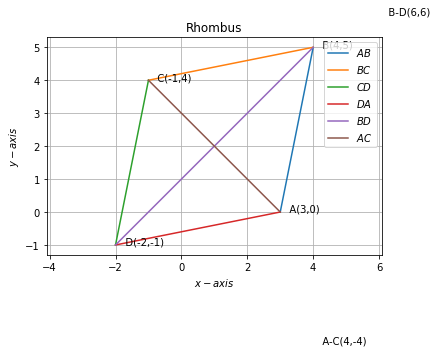
\includegraphics[width=\columnwidth]{./figs/fig.png}
 \end{center}
\caption{}
\label{fig:Fig1}
\end{figure}
\end{enumerate}

\end{document}